% !TeX root = Report.tex
\section{Project Management}

\subsection{Methodology}

The requirements of the project were not fully understood at the beginning of it and we were unsure of the efficiency of our algorithms we were developing, therefore, we used a prototyping approach as part of an evolutionary process model \cite[p.~42--44]{pressman2010software}. This allowed us to start with a set of core requirements and then incorporate other extensions as the requirements are better understood. We had meetings with our supervisor to discuss the best ways to implement our system and any what additional components we should start developing. When a new idea was defined, a prototype was modelled, constructed and tested. For some parts of the project we sought out our supervisors advice as to how to implement it or what new approach we could try to take. The process was repeated until we had a sufficiently stable base of libraries and the intended code developed.

\subsubsection*{Term 1}

We spent the first few weeks researching on the different aspects of wireless sensor networks as well as the appropriate tools and platform to develop our system with. Much of this involved installing and setting up the software and then developing simple applications with it to learn how the system works and how to develop for it. Much of the group was learning this from scratch, making this a slow and difficult part of the project. We focused on developing a single algorithm (PELP) and the framework that required, with the intent to extend it later. Due to the large number of algorithms we intend to implement, we made a list of such algorithms and implemented the most relevant ones first. As we progressed through the development, the list was updated by removing or adding algorithms that had been implemented or still needed to be implemented.

\subsubsection*{Term 2}

At this stage, most of the algorithms and protocols were implemented independently and treated as individual components to the core system. We decided to do it this way because of the benefits of modularity where the principles of ``Separation of Concerns'' \cite[p.~99]{pressman2010software} allows for a more manageable set of modules. The composition of these components such as predicate checking and neighbour data retrieval was done during the entire winter vacation and the beginning of the second term.
%We can mention here a small list of the algorithms that needed to be integrated together

In the second term, we continued following the evolutionary process model but at a more relaxed approach which focuses on finishing the system components and preparing the gathering of results. Since the project scope was clear and we had a more directed goal, fewer meetings with the supervisor was needed as we simply needed to implement modules. We still had meetings with our supervisor, however, they were less frequent than in the first term. Ensuring that the development and debugging phase could be completes in time required the effective scheduling of tasks and prioritising work. Unfortunately, by the second half of the term, progress had fallen to a halt due the high number of coursework deadlines and this meant that team members where preoccupied with other duties. To address the issue, a meeting was held prior to the halt where we discussed our recovery plan and actions to take once members was free. This allowed team members to continue working where they left off and avoid any delays. However, it was not until during the Easter holiday that the project gained the momentum to finish development and results gathering.

\subsection{Role Allocation}

We decided to allocate roles in the second week after we had the first week to perform research into the problem and find out what has been done. The following were how we assigned roles, although we intend for these to be flexible:

\begin{table}[H]
\centering
	\begin{tabular}{| c | c |}
		\hline
		Name & Role\\
		\hline
		Matthew Bradbury & Group Leader\\
		Daniel Robertson & Project Manager\\
		Amit Shah & Technical Leader\\
		Ivan Leong & Developer and Tester\\
		Joe Yarnall & Developer and Tester\\
		Tim Law & Developer and Researcher\\
		\hline
	\end{tabular}
\end{table}

Whilst the entire team was responsible for system design and development, it was critical to have a group leader and other leading roles to facilitate and provide resources to the team. Their individual responsibilities were as follows:

\begin{itemize}
	\item[] {\bf Matthew Bradbury} - Group Leader
	
	His main task was to lead the entire project and have a clear understanding of the components that is to be implemented. He is responsible for allocating tasks to its team members and providing direction for meeting the project objectives. He also possesses strong communication skills with his team members as well as being able to explain the concepts to the supervisor concisely. Ensures that everyone is performing their roles accordingly and providing motivation when the project is slowing down.	

	\item[] {\bf Daniel Robertson} - Project Manager
	
	He supported the group leader by facilitating the management of the project and ensuring that the overall work is done on schedule. He arranges weekly meetings and provides a summary report prior to each meeting and records all discussions.
	
	\item[] {\bf Amit Shah} - Technical Leader
	
	Responsible for overseeing the work done by other members and ensures that all code written by the team meets the technical specification and design requirements of the project. Also responsible for looking after the hardware and the development with it.
	
\end{itemize}

\subsection{Project Planning}

Our initial planning was done in the first few group meetings and most of the plan details was explained in the project specification. As we progressed through the project development, we encountered many changes from the initial plan as well as changes in task schedule. This section presents the final overall plan of the project including the revised time schedule of development activities, resources used and issues encountered.

\subsubsection{Work Breakdown Structure}

The figure below shows the work breakdown structure as designed for the project specification.

\begin{figure}[H]
\centering
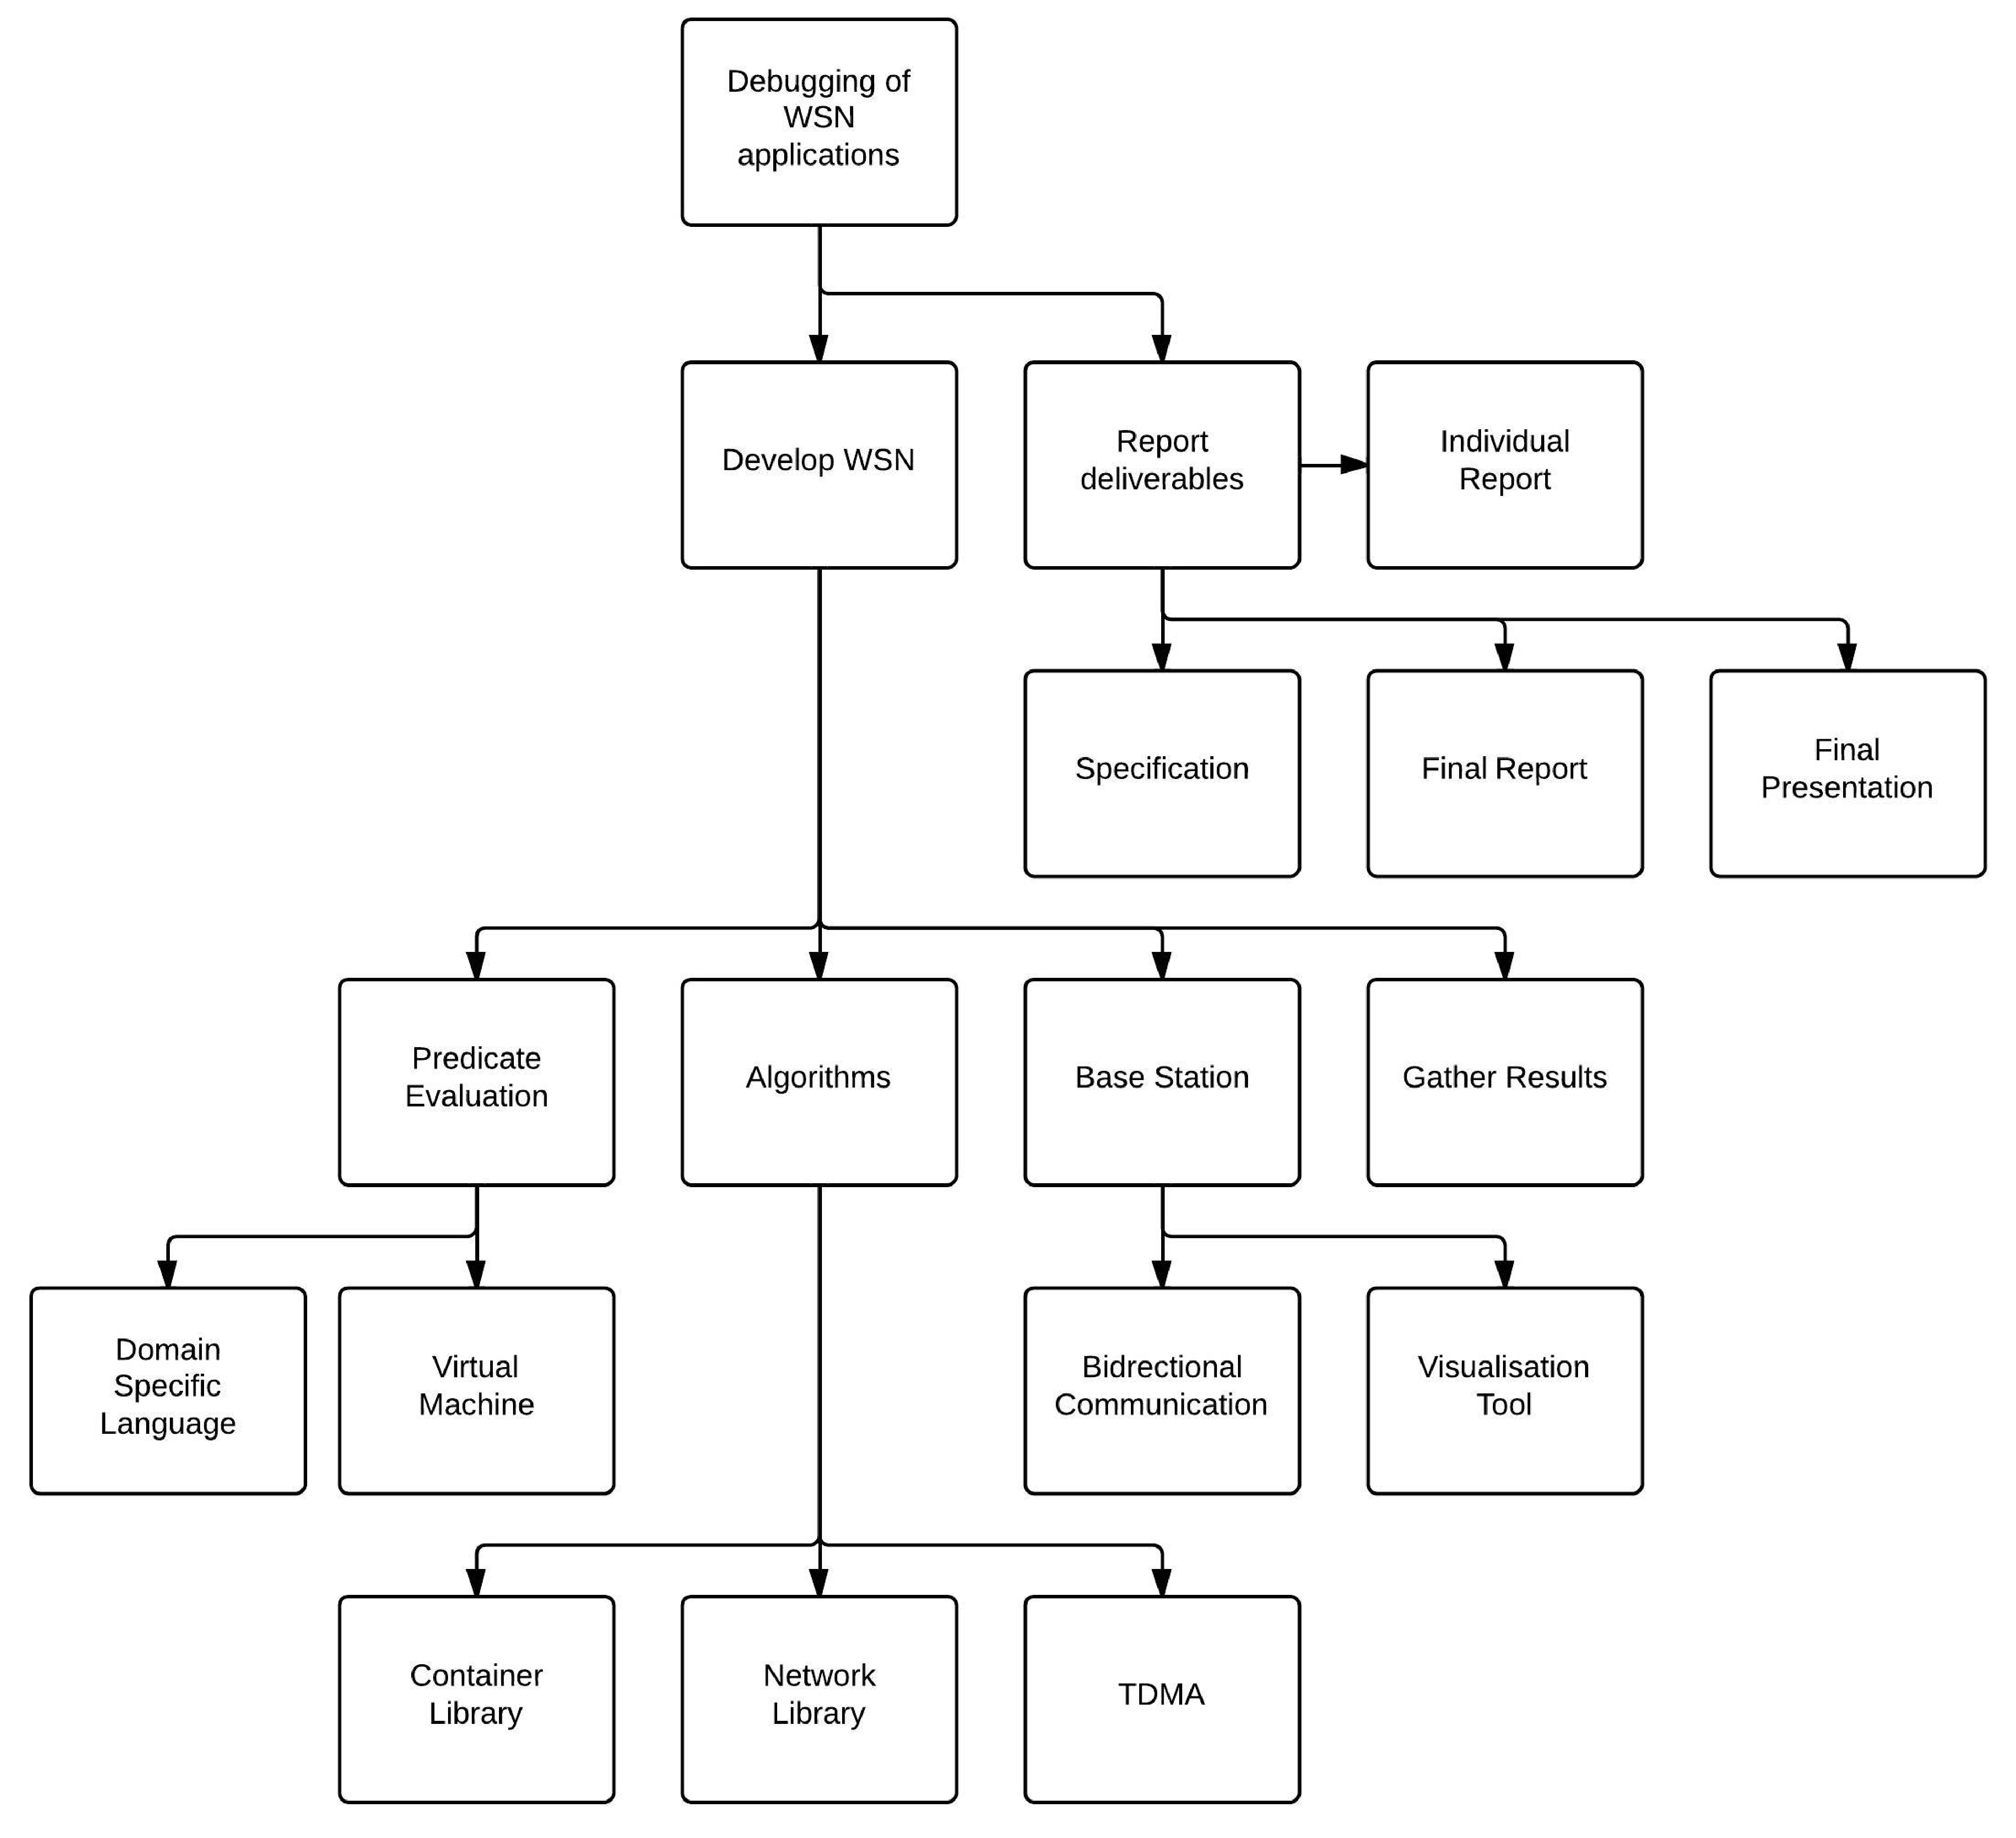
\includegraphics[width=\linewidth]{Images/pm-wbs.pdf}
\caption{Work Breakdown structure}
\label{fig:Work Breakdown Structure}
\end{figure}

\subsubsection{Deliverables}

Our project consists of 5 deliverables which includes one individual report. It was very important that these milestones were met because it allows us to monitor our progress and prove that we were working in the direction of the stated goals and requirements of the project.

\begin{enumerate}
	\item Specification \emph{(Due Week 4 - Term 1)}
	
	This was the first deliverable of the project. At the time, we were still undergoing research on the different components of the system and the project scope was not clearly defined. Nevertheless, we highlighted in the specification the main goals of our project and the different algorithms that we wished to implement. We also included a schedule of all the planned activities for the remainder of the project and an approximate time taken to complete them.
	
    \item Progress Poster Presentation \emph{(Due Week 10 - Term 1)}
    
	By the end of the first term, the scope of the project had reached a more defined level as we had decided what is to be implemented and what has been disregarded from the provisional list of algorithms. This was demonstrated in our first delivery - the poster presentation, where we had to chance to explain our project at a high level to our supervisors and other professors.
    
    \item Final Group Report \emph{(Due Week 1 - Term 3)}
    
	Although the report is due in term three we started adding content since the first term. This included the introduction, literature review, a list of algorithms and protocols to be implemented and a brief description of their functions. In the beginning of the second term, much of the algorithms were described in the report and it was only towards the end of the term that the report was being updated on a full scale. Each member was assign a specific section to work on but with the flexibility to update other sections if it was related to them.
	
    \item Individual Report \emph{(Due Week 1 - Term 3)}
    
	Every team member needs to write a 3000 words report to reflect on their performance and contribution towards the project as an individual.
    
    \item Final Project Presentation \emph{(Due Week 3 - Term 3)}
    
    Demonstrate our final project to a panel of judges and our supervisor.
 
\end{enumerate}

\subsubsection{Schedule}

Throughout the term, every member was assigned specific tasks and was given a time frame to complete them. The table below shows the time schedule allocated to each members.

\begin{table}[H]
	\centering
	\begin{tabular}{| l | l | l | l | l | l | l |}
	\hline
	Task Description & \multicolumn{6}{l|}{Time Allocated (Weeks)}\\
	~ & Amit & Dan & Ivan & Joe & Matt & Tim \\
	\hline
	\hline
	\multicolumn{7}{|l|}{\textbf{Term 1} - Developing for application predicate checking} \\
	\hline


	Research around the Problem & 2 & 2 & 2 & 2 & 2 & 2\\
	Writing Specification & 1 & 1 & 1 & 1 & 1 & 1\\
	H-SEND Implementation & 3.5 & ~ & ~ & 3.5 & ~ & ~\\
	``Send to Base'' Implementation & ~ & ~ & ~ & ~ & 2 & 1.5\\
	Clustering Implementation & ~ & 3.5 & 2 & ~ & ~ & ~\\
	Aggregation Tree Implementation & ~ & ~ & ~ & ~ & 1.5 & ~\\
	Develop Visualisation Tool & ~ & ~ & 1.5 & ~ & ~ & 2\\
	Develop Predicate Language Runtime & ~ & ~ & ~ & ~ & ~ & 2\\
	Testing and Adapting to Physical Nodes & 2 & 2 & 2 & 2 & 2 & 2\\
	Message Logging & ~ & ~ & ~ & 1 & ~ & ~\\
	Poster Creation and Presentation preparation & 1.5 & 1.5 & 1.5 & 1.5 & 1.5 & 1.5\\

	\hline
	\hline
	\multicolumn{7}{|l|}{\textbf{Term 2} - Developing for network predicate checking and where the predicate is checked} \\
	\hline
	
	Additional Research & 1 & 1 & 1 & 1 & 1 & 1\\
	Improving Dynamic Predicate Specification & 2 & 2 & ~ & ~ & 2 & 2\\
	Develop Visualisation Tool & 2 & ~ & 2 & 2 & ~ & 2\\
	Modify Algorithms to Selectively Evaluate Predicates & ~ & 2 & 2 & 2 & 2 & ~\\
	Performance Testing & 1.5 & 1.5 & 1.5 & 1.5 & 1.5 & 1.5\\
	Testing and Adapting to Physical Nodes & 1.5 & 1.5 & 1.5 & 1.5 & 1.5 & 1.5\\
	Report Writing & 2 & 2 & 2 & 2 & 2 & 2\\
	\hline
	
	\end{tabular}
\end{table}

\subsubsection{Gantt Chart}

The project plan was adhered to as much as possible and was closely monitored as shown in the Gantt chart below. The Gantt chart was edited several times and accounted for revisions made whenever there was a change in task or time schedule. The colours of the bars are as follows:

\begin{itemize}
	\item[] Green: Research and learning
	\item[] Orange: Design
	\item[] Blue: Implementation
	\item[] Yellow: Specification and report preparation
	\item[] Red: Testing
\end{itemize}

\begin{figure}[H]
\centering
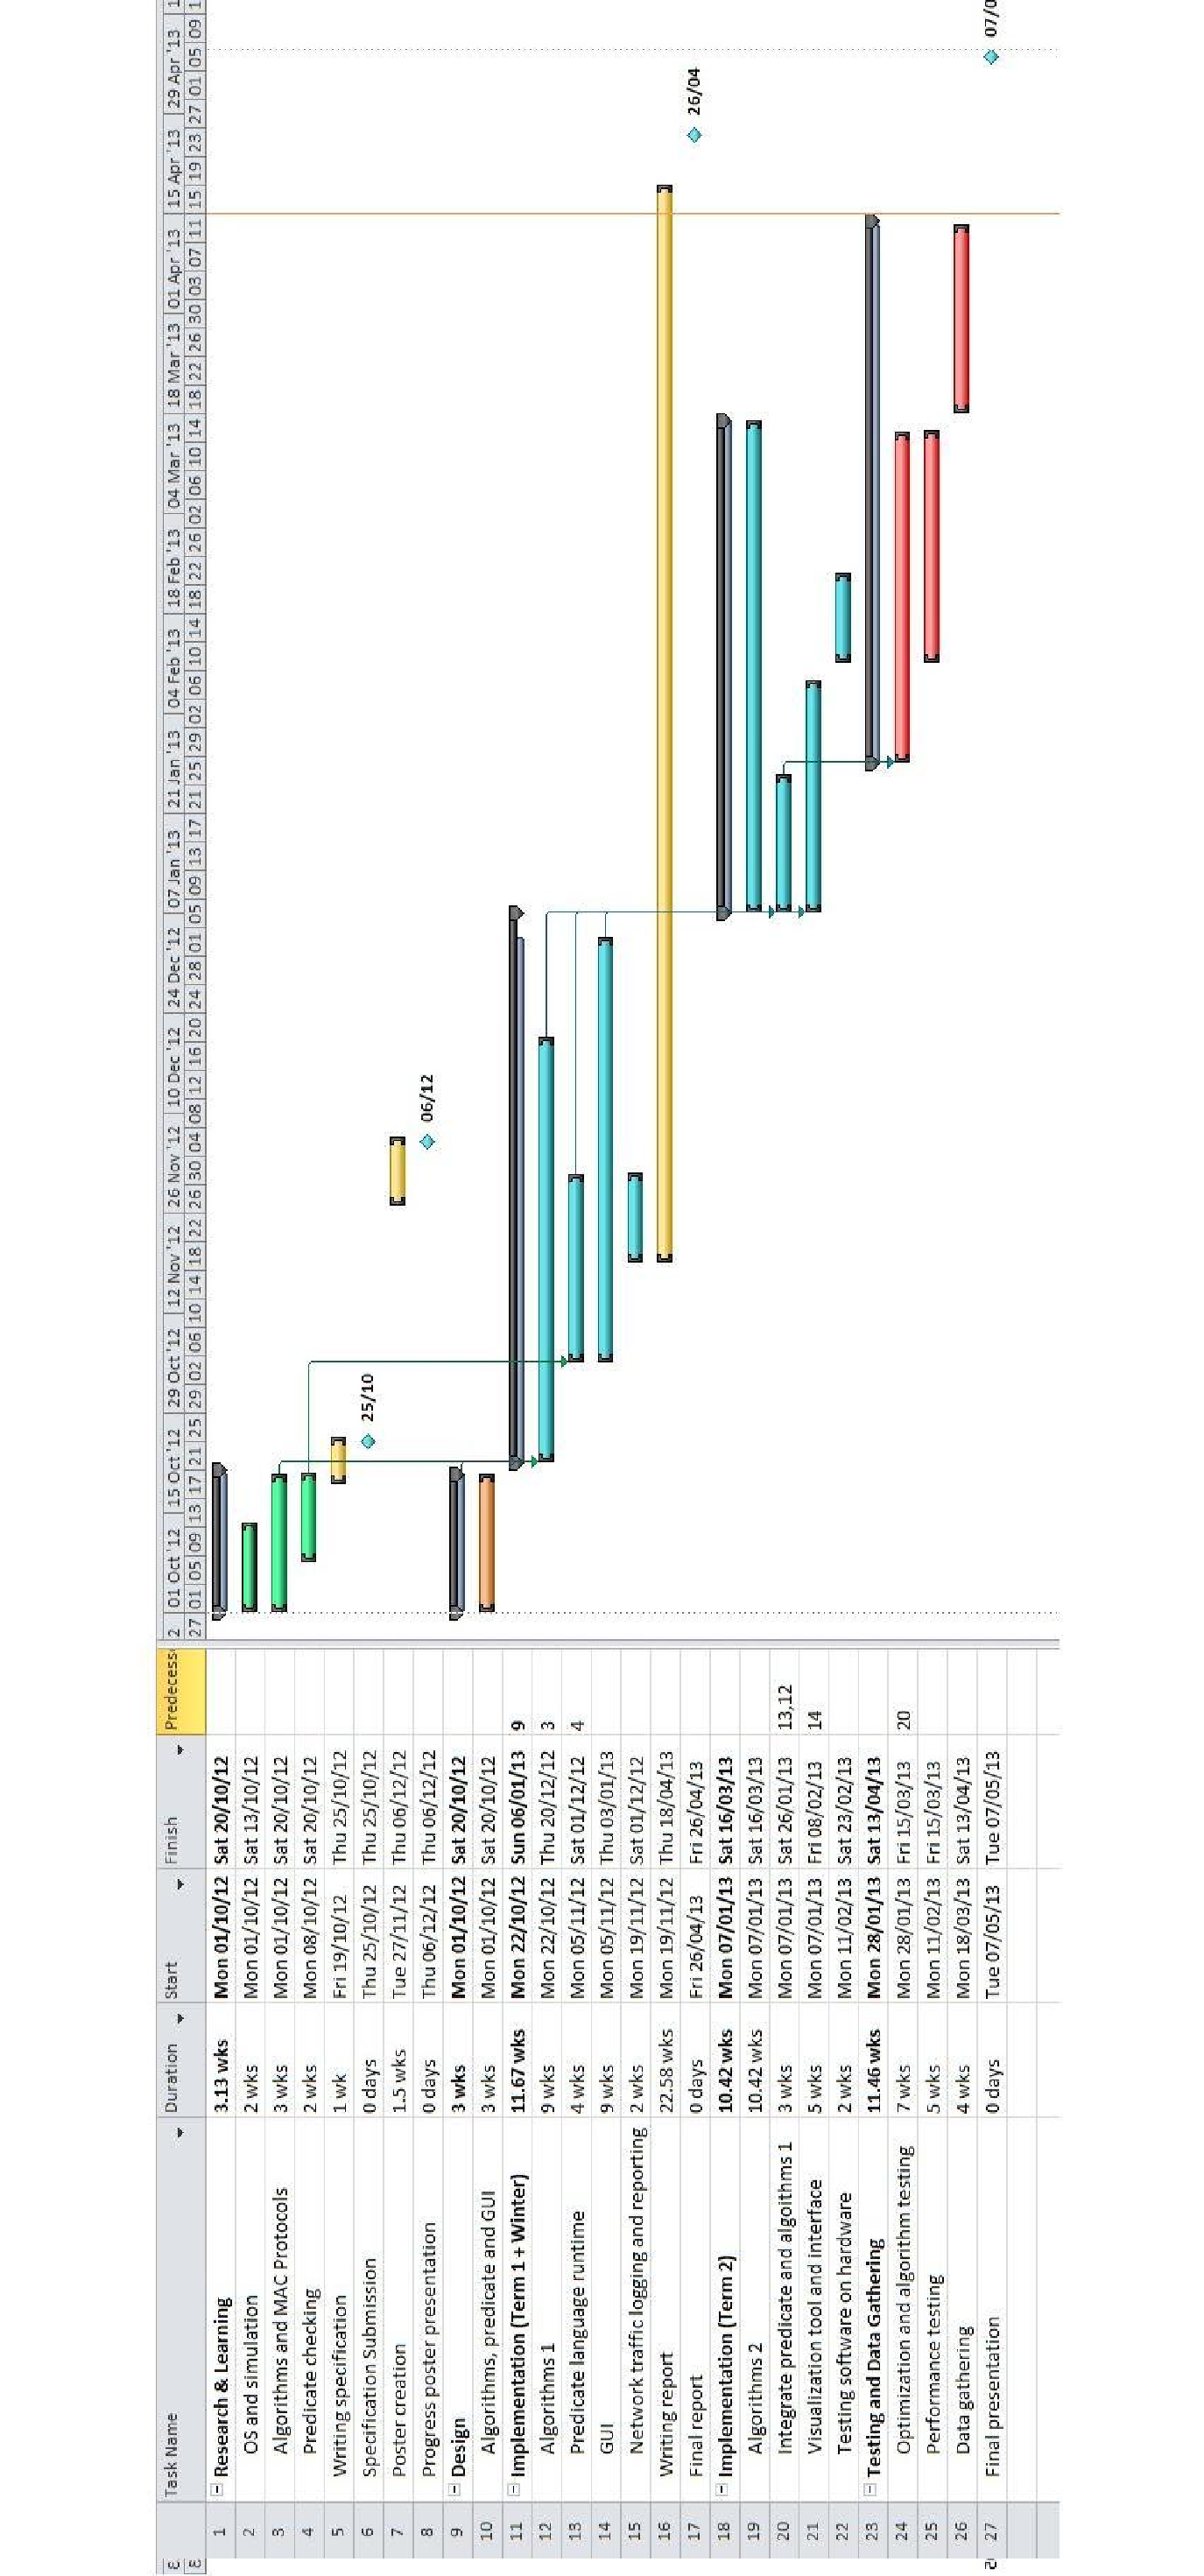
\includegraphics[height=.99\textheight]{Images/pm-gantt.pdf}
\caption{Gantt Chart}
\label{fig:Gantt Chart of project}
\end{figure}

\subsection{Resources}
% Can explain more on the software we used to share resources, communicate and discuss ideas.

\subsubsection{Source Control Management}

We signed up for a Git repository on BitBucket \cite{bitbucket} where we committed all the work we produced. We initially had an issue that free private repositories hosted on BitBucket have a maximum of 5 participants, whereas we had 6 group members. Fortunately when new users sign up to the services from an invite, the person that sends the invite gets additional capacity. This meant that the person who created the repository ended up with enough capacity for all members to access the account. The use of BitBucket also gives the advantage of branching and merging codes from different users without needing to replicate any files and worry about redundancy. 

\subsubsection{Communication}

When group members are working online, the main source of communication is via the popular social networking platform - Facebook. We created a group for our team where members could post any messages regarding the project such as issues in code development, assignment of tasks to team members and reminders of any project activities (e.g. weekly meetings).

\subsubsection{Development tools}

The following table summaries all the software and hardware used to develop the wireless sensor network application. 

%To add more items increment multirow

\begin{table}[H]
\centering
\begin{tabular}{| l | p{2.5cm} | p{4.5cm} | p{4.25cm} |}
	\hline
	~ & Name & Description & Constraints/Issues\\
	\hline

	\multirow{13}{*}{Software} & Contiki & Operating System for WSNs & ~
	
	\\ \cline{2-4}

	& Cooja & Contiki Simulator & ~
	
	\\ \cline{2-4}

	& Bash and Python & Scripting numerous tasks & Some dependencies had to be manually installed\\ 
	\cline{2-4}

	& Make & To compile the C source code for the project & ~\\ 
	\cline{2-4}

	& MSP-GCC & The custom compiler used & Did not come installed on DCS computers, needed to compile ourselves\\ 
	\cline{2-4}

	& Netbeans and Java & To develop the GUI & ~\\ 
	\hline

	\multirow{7}{*}{Hardware} & Sensor nodes & See \autoref{sec:dev-spec} & Provided by department, needed to share with PhD student who also required them\\ 
	\cline{2-4}

	& USB Hub and USB cables & To work with multiple sensor nodes at once & Hub required purchasing, cables were borrowed from DCS\\
	\cline{2-4}
	
	\hline
\end{tabular}
\end{table}


\subsection{Risk Analysis}
%Potentially the issues below can form part of risk
It is almost certain that every project contains risks which could impact its progress and success if not well managed. Risk management involves two basic steps, 1) to identify the different possible risks that may occur in the project and its likelihood of occurrence and 2) state the actions to mitigate the effects of any threats. \autoref{tab:risk} contains a number of risks that we considered and how we planned to mitigate their effect. We also ranked them by severity and likelihood so we know which risks we needed to prioritise mitigation and which we needed to be on the watch for, where 1 represents the least severe or least likely and 10 represents the most severe or most likely.

\begin{table}[H]
\centering
\begin{tabular}{| p{4cm} | l | l | p{7cm} |}
	\hline
	Risk & Likelihood & Severity & Mitigation\\
	\hline	
	
	Personal Hardware and Software failure (i.e. personal computers)
	\begin{itemize}
		\item Report and research
		\item Software code
	\end{itemize}
	 & 2 & 9 & To prevent the risk of data lost, we used a Bitbucket repository to save and store all our documents and program coding online. This also allows the concurrent development of our project and ensuring that all team members are up to date.
	 
	\\ \hline
	
	Team member illness and absence
	& 5 & 4 & There would be circumstances where team members would be unavailable to work on the project for a short period of time. To ensure that work is progressive, necessary measures were taken. For example an absent member can temporary delegate his current task to a different member. Code should also be well documented to allow others to take over work on it.
	
	\\ \hline
		
	Meeting deadlines and schedules
	& 5 & 7 & It was important that every milestone of the project was met so that no marks were penalised. The progress of the project was monitored and we had weekly meetings to ensure that everyone was on track of their given tasks.
	
	\\ \hline
	
	Obtaining desired results when deploying code (tested on simulated environment) on physical devices
	& 5 & 4 & Most of the code that was developed in the beginning was tested with the Cooja simulator. It would be unlikely to obtain similar results when deployed on the actual hardware due to a wide range of environmental factors such as interference and power distribution. An option is to gather data from simulated environment rather than physical devices.
	
	\\ \hline
		
	Defining the scope of our project
	& 6 & 7 & There are many issues and research problems that revolve around the topic of wireless sensor networks. It is important to define the scope of the project to prevent scope creep and necessary expansion of the project.

Need to keep track of all new ideas proposed by the supervisor and raise any change requests to the project.

	\\ \hline
		
	Damage of the sensor nodes
	& 2 & 8 & Each of the sensor nodes cost 80 Euros. The sensors must be handled with care to prevent any cost of damage. Assign a group member the responsibility to store the sensors after use and keep track of who is using them.
	
	\\ \hline
		
	Components of the project that could not be implemented with current tools.
	& 4 & 4 & Research on alternative methods or implement custom tools.
	\\ \hline
\end{tabular}
\caption{Risk analysis}
\label{tab:risk}
\end{table}

\subsection{Work Overview}

This section highlights the different tasks that was undertaken by each group member for every week of term 1 and term 2. At every weekly meetings, the project leader would discuss the progress of the tasks that was assigned in the previous week and any new tasks for the current week would be recorded as shown in the table below.
%perhaps number the table below 

\subsubsection*{Term 1}

\begin{center}
	\begin{longtable}{| l | p{9cm} | p{3.5cm} |}
	\hline
	Week & Activities & Task Allocation\\
	\hline
	1 & \begin{enumerate}
			\item Meet up with Supervisor and discuss project direction
			\item Research on related work and what we can develop, before settling on main aims
			\item Investigate two OS and their corresponding simulators: TinyOS with TOSSIM and Contiki with Cooja
		\end{enumerate} &
	\begin{enumerate}
		\item[] Amit: All
		\item[] Dan: All
		\item[] Ivan: All
		\item[] Joe: All
		\item[] Matt: All
		\item[] Tim: All
	\end{enumerate}
	\\ \hline

	2 & \begin{enumerate}
			\item Research if Cooja can be extended through the use of plug-ins (with the aim of extending it to replay traffic logs)
			\item Research Clustering algorithms and find implementations
			\item Develop a temperature dissemination application to learn Contiki and Cooja
			\item Research TinyOS and TinyDB and see if they could be applied to predicate checking
			\item Investigate performance of different MAC protocols
			\item Investigate the feasibility of live monitoring of the network
			\item Investigate QoS and how it may be applied to real life WSN deployments
			\item Produce a literature review on chosen topic
		\end{enumerate} &
	\begin{enumerate}
		\item[] Amit: 1, 7, 8
		\item[] Dan: 5, 8
		\item[] Ivan: 6, 8
		\item[] Joe: 4, 8
		\item[] Matt: 3, 8
		\item[] Tim: 2, 8
	\end{enumerate}
	\\ \hline
	
	3 & \begin{enumerate}
			\item Research DICAS
			\item Research Send to Base
			\item Research Daicon
			\item Research DIDUCE
			\item Research H-SEND
			\item Research Sympathy
			\item Write Specification
		\end{enumerate} &
	\begin{enumerate}
		\item[] Amit: 2, 7
		\item[] Dan: 4, 7
		\item[] Ivan: 3, 7
		\item[] Joe: 1, 7
		\item[] Matt: 6, 7
		\item[] Tim: 5, 7
	\end{enumerate}
	\\ \hline
	
	
	4 & \begin{enumerate}
			\item Finish Specification
			\item Work out how to get MSP430-GCC and the Cooja working on Joshua
			\item Begin developing aggregation tree example
		\end{enumerate} &
	\begin{enumerate}
		\item[] Amit: 1, 2
		\item[] Dan: 1
		\item[] Ivan: 1
		\item[] Joe: 1
		\item[] Matt: 1, 3
		\item[] Tim: 1
	\end{enumerate}
	\\ \hline
	
	
	5 & \begin{enumerate}
			\item Get used to developing in C and learn how to use the Contiki libraries
			\item Finish developing aggregation tree
			\item Start implementing clustering algorithms
			\item Start implementing H-SEND
		\end{enumerate} &
	\begin{enumerate}
		\item[] Amit: 1, 4
		\item[] Dan: 1, 3
		\item[] Ivan: 1, 3
		\item[] Joe: 1, 4
		\item[] Matt: 1, 2
		\item[] Tim: 1
	\end{enumerate}
	\\ \hline
	
	
	6 & \begin{enumerate}
			\item Start Implementing GUI
			\item Implementing clustering algorithms (Regular and Hierarchical)
			\item Implement H-SEND
			\item Implement a local predicate checker and reporter
		\end{enumerate} &
	\begin{enumerate}
		\item[] Amit: 3
		\item[] Dan: 2
		\item[] Ivan: 2
		\item[] Joe: 3
		\item[] Matt: 4, 2
		\item[] Tim: 1
	\end{enumerate}
	\\ \hline
	
	7 & \begin{enumerate}
			\item Library-ify Cluster implementations
			\item Implement LEACH  using existing implementations as a base
			\item Work out how to interface the GUI and the base station
			\item Continue developing GUI
			\item Get in contact with Sain Saginbekov and sort out when we can use sensor nodes
			\item Contact Victor Sanchez and inform him when we are using sensor nodes
			\item Implement multi-hop predicate checking
			\item Slim down eLua enough for us to run it on the sensor nodes, to allow for dynamic predicate specification
			\item Research and start implementing network traffic logging and reporting
		\end{enumerate} &
	\begin{enumerate}
		\item[] Amit: 7
		\item[] Dan: 1, 2
		\item[] Ivan: 9
		\item[] Joe: 5, 6, 7
		\item[] Matt: 8
		\item[] Tim: 3, 4
	\end{enumerate}
	\\ \hline
	
	8 & \begin{enumerate}
			\item Start work on poster with the aim of finishing it by the end of week 9
			\item Detect and report neighbours for display in the visualisation tool, aim to be able to work in mobile networks, with gained and lost neighbours
			\item Log network data and report it to the network (for visualisation tool to replay traffic)
			\item Finish predicate language parser and code generation
			\item Tidy up n-hop HSEND
			\item Integrate n-hop HSEND with predicate language virtual machine
			\item Experiment with interference affecting node communications
		\end{enumerate} &
	\begin{enumerate}
		\item[] Amit: 1, 5, 6
		\item[] Dan: 1, 3, (~7)
		\item[] Ivan: 1, 2, (~7)
		\item[] Joe: 1, 2, (~7)
		\item[] Matt: 1, 4, 6
		\item[] Tim: 1, 4
	\end{enumerate}
	\\ \hline

	9 & \begin{enumerate}
			\item Create poster for presentation
		\end{enumerate} &
	\begin{enumerate}
		\item[] Amit: 1
		\item[] Dan: 1
		\item[] Ivan: 1
		\item[] Joe: 1
		\item[] Matt: 1
		\item[] Tim: 1
	\end{enumerate}
	\\ \hline

	10+ & \begin{enumerate}
			\item Code generation for predicate language
			\item Network visualisation (node neighbours)
			\item GUI to Node interface
			\item Message logging
			\item Neighbour Reporting
			\item Turn existing code into libraries
			\item Make existing code handle generic data
			\item Integrate predicate evaluating VM and neighbour data retrieval
			\item Write up notes on work done this term
		\end{enumerate} &
	\begin{enumerate}
		\item[] Amit: 6, 7, 8, 9
		\item[] Dan: 4, 5, 9
		\item[] Ivan: 3, 5, 9
		\item[] Joe: 6, 7, 8, 9
		\item[] Matt: 6, 7, 8, 9
		\item[] Tim: 1, 2, 9
	\end{enumerate}
	\\ \hline
	
	\end{longtable}
\end{center}

\subsubsection*{Term 2}

\begin{center}
	\begin{longtable}{| l | p{7.5cm} | p{5cm} |}
	\hline
	Week & Activities & Task Allocation\\
	\hline
	1 - 2 & \begin{enumerate}
		\item Continue network visualisation
		\item Interface Base station node with desktop application
		\item Develop neighbour detection and reporting to sink
		\item Integrate predicate evaluating, predicate VM and neighbour data retrieval
		\item Finish parser and compiler of predicate language
		\end{enumerate} &
	\begin{enumerate}
		\item[] Amit: 4
		\item[] Dan: 3
		\item[] Ivan: 2
		\item[] Joe: 4
		\item[] Matt: 4, 5
		\item[] Tim: 1
	\end{enumerate}
	\\ \hline

	3 & \begin{enumerate}
		\item Continue network visualisation
		\item Interface Base station node with desktop application
		\item Develop type checker for predicate language
		\item Find bug that is causing unicast communications to fail
		\item Develop a way to handle packets larger than the maximum broadcast size
		\end{enumerate} &
	\begin{enumerate}
		\item[] Amit: 4
		\item[] Dan: 5
		\item[] Ivan: 2
		\item[] Joe: 4
		\item[] Matt: 3
		\item[] Tim: 1
	\end{enumerate}
	\\ \hline

	4 & \begin{enumerate}
		\item Continue network visualisation
		\item Interface Base station node with desktop application
		\item Find bug that is causing unicast communications to fail
		\item Develop a way to handle packets larger than the maximum broadcast size
		\item Develop some containers for use in our applications (lists and maps)
		\end{enumerate} &
	\begin{enumerate}
		\item[] Amit: 3
		\item[] Dan: 4
		\item[] Ivan: 2
		\item[] Joe: 3
		\item[] Matt: 3, 5
		\item[] Tim: 1
	\end{enumerate}
	\\ \hline

	5 & \begin{enumerate}
		\item Continue network visualisation
		\item Interface Base station node with desktop application
		\item Improve reliability of application on physical hardware
		\item Refactor N-Hop-Req to split up request and reply phases
		\item Develop a way to handle packets larger than the maximum broadcast size
		\item Optimise and debug Tree Aggregation and Predicate Checking
		\end{enumerate} &
	\begin{enumerate}
		\item[] Amit: 3, 6
		\item[] Dan: 5
		\item[] Ivan: 2
		\item[] Joe: 4
		\item[] Matt: 6
		\item[] Tim: 1
	\end{enumerate}
	\\ \hline

	6 - 10 & \begin{enumerate}
		\item Implement nhopflood
		\item Implement Event based data sending
		\item Implement Event-based predicate evaluation (PELE, PEGE)
		\item Implement Global predicate evaluation (PEGP, PEGE)
		\item Implement GUI
		\item Get bidirectional communications between motes and desktop working
		\item Develop a way to handle packets larger than the maximum broadcast size (multipacket)
		\item Debug and Test
		\item Implement failure responses for predicate evaluation
		\item Run simulations to gather results
		\end{enumerate} &
	\begin{enumerate}
		\item[] Amit: 3, 4, 8, 9, 10
		\item[] Dan: 1, 7, 8
		\item[] Ivan: 6, 8
		\item[] Joe: 8, 9
		\item[] Matt: 1, 2, 3, 4, 6, 7, 9, 10
		\item[] Tim: 5, 8
	\end{enumerate}
	\\ \hline
	
	\end{longtable}
\end{center}


\subsection{Management Issues}

\subsubsection{Group Members Without Internet}
Unfortunately two of our group members were without internet for the first 3 weeks of term. This was an issue because they were unable to just work in the DCS labs because the computers there didn't have the software required (such as VirtualBox or the WSN simulators). To work around this, those two members were given tasks that could be accomplished with their own machines and without internet. Once they obtained internet they were given tasks, that access allowed them to accomplish.

\subsubsection{Society Exec Clashes}
Two members of our team are on the exec of Warwick Societies, this means that at certain parts of the year they were in high demand for those jobs. For instance during the first few weeks of term during Freshers' Fortnight, the exec members were required to be involved in many of their events that they were running. Also during a large section of term 2, there were a number of events that required their presence such as exec elections and the Battle of the Bands. Between these busy periods the demand on their time decreased and made balancing the time been the demands of this project and their exec roles much easier.

\subsubsection{High Number of Coursework Deadlines in Term 2}
In the second term, there where many coursework deadlines for other course modules and some of the team members were unable to contribute towards the project for some periods of time due to increased workload. On several occasion, the team leader had to put pressure on the team to ensure that some time was delegated to project work. 

\subsection{Legal and Professional Issues}

This project involves working with open source code and libraries, so the use of this code must follow the requirements of the licences of that code. Ideally we would wish to contribute some of what we have developed back to the open source community as we feel that some of it may be of use. We intend to clarify the ownership of the code and will look into sorting out the legalities of contributing it back to the Contiki OS project.

%Just brief notes
%\begin{enumerate}
%	\item Our project practice complies with the ACM code ethics and professional conduct.
%	\item We aim to contribute some of the work back to the WSN community or to whom it may be of interest. However there may be issues with university regulations regarding the ownership of our code.
%	\item Legality of copyright with respect to the owners of the source code. (Licence agreements)
%\end{enumerate}

